\setcounter{chapter}{1}
\chapter{Magnetostatica}

\section{Correnti stazionarie}

Le cariche generano campi elettrici. Le correnti di cariche generano campi magnetici. Restringiamo lo studio al caso in cui la densit\`a di carica \`e $\rho = 0$, in modo tale che $\bold{E} = 0$ e quindi possiamo concentrarci solo sul campo magnetico. 

Dato che per ipotesi $\rho = 0$, non pu\`o esserci carica netta, questo vuol dire che cariche positivi e negative si bilanciano tra loro in ogni punto dello spazio. Inoltre, dato che le cariche possono muoversi \`e presente una corrente anche se non c'\`e un trasporto netto di carica.
\newline

Sembrer\`a strano, ma \`e esattamente quello che succede all'interno di un normalissimo filo. Questo \`e dovuto al fatto che ci sono delle cariche positive libere nel metallo per via del reticolo di ioni, ma dato che si muovono tutti insieme riusciamo ad avere in ogni singolo punto una densit\`a di carica nulla. L'\textit{equazione di continuit\`a}, che descrive la conservazione della carica \`e data da, 
\begin{equation}
	\frac{\partial \rho}{\partial t} + \nabla \cdot \bold{J} = 0
\end{equation}
e dato che la densit\`a di carica \`e costante, diventa 
\begin{equation*}
	\nabla \cdot \bold{J} = 0
\end{equation*}
Matematicamente vuol dire che se abbiamo un flusso di corrente in una certa regione di spazio, un eguale corrente deve fluire in senso opposto affinch\`e non ci sia un addensamento di carica. Notare che questo \`e consistente con la propriet\`a che per ogni campo vettoriale si ha che $\nabla \cdot (\nabla \times \bold{B}) = 0$.

\subsection{Derivzione dell'equazione di continuit\`a}

Per caratterizzare il trasporto di carica si introducono alcune grandezze fisiche. Una delle prime \`e \textit{l'intensit\`a di corrente:}
\begin{equation*}
	I = \frac{dq}{dt}
\end{equation*} 
che descrive la quantit\`a di carica netta che attraversa ala sezione di un mezzo in unit\`a di tempo. La unit\`a di misura in cui viene espressa \`e data dall`\textit{Ampere} che esprimiamo come
\begin{equation*}
	[A] = \frac{[ Coulomb]}{[ Secondi]}
\end{equation*}
La definizione pu\`o essere generalizzata al trasporto di carica nello spazio, riconducendola ad una grandezza vettoriale e al concetto di flusso attraverso una superficie.
\begin{wrapfigure}{r}{0.4\textwidth}  % r for right alignment, 0.4 is the width of the figure
    \centering
    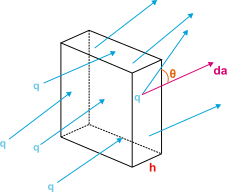
\includegraphics[width=0.4\textwidth]{images/fluxden}  % Include your image here
\end{wrapfigure}

La seconda grandezza che andiamo ad introdurre \`e la \textit{densit\`a di corrente}, questa \`e legata ad un volume generico costituito da un materiale al cui interno le cariche siano libere di muoversi in una direzione generica. Ipotizziamo di avere nel mezzo dei portatori di carica tutti identici tra loro, identificati dalle seguenti grandezze comuni:

\begin{enumerate}
	\item $n_q \rightarrow$ densit\`a di portatori di carica per unit\`a di volume ;
	\item $q \rightarrow $ carica dei portatori;
	\item $\bold{v} \rightarrow $ velocit\`a di spostamento delle cariche;
	\item $\bold{da} \rightarrow$  elemento infinitesimo di superficie del volume.  
\end{enumerate} 
Dato il parallelepipedo in figura solo le cariche al suo interno di base $da$ e altezza $h = v \Delta t \cos \theta $ attraversano la superficie in un intervallo di tempo $\Delta t$.

Di conseguenza la variazione di carica attraverso la superficie $\bold{da}$ \`e data dalla relazione 
\begin{equation*}
	\Delta Q = n \;q\; da \; h = n\; q \;v \Delta t \cos \theta da = n \;q \; \bold{v} \cdot \bold{da} \; \Delta t 
\end{equation*}
La corrente attraverso $\bold{da}$ \`e associata al flusso della grandezza $n_q \bold{v}$, da cui possiamo definire 
\begin{equation*}
	dI = \lim_{\Delta t \to 0} \frac{\Delta Q}{\Delta t} = nq \bold{v} \cdot \bold{da} 
\end{equation*}
Nel caso pi\`u generico all'interno del volume possono esistere diversi portatori di carica $q_i$, con velocit\`a differenti $\bold{v}_i$, dunque per ciascuna specie di particella possiamo definire 
\begin{equation*}
	dI_i = (n_iq_i\bold{v}_i)\cdot \bold{da}
\end{equation*}
e di conseguenza la corrente infinitesima complessiva \`e 
\begin{equation*}
	dI = \sum_{i}dI_i = \left (\sum_{i}n_i q_i \bold{v}_i \right) \cdot \bold{da}
\end{equation*}
dove definiamo la grandezza vettoriale
\begin{equation*}
	\bold{J}= \sum_{i}n_i q_i \bold{v}_i 
\end{equation*}
\textit{densit\`a di corrente}, che \`e identificata dalle unit\`a di misura 
\begin{equation*}
	[\bold{J}] = [I \; L^{-2}] = \frac{Ampere}{m^2}
\end{equation*}
Non \`e necessario che tutte le cariche dello stesso tipo abbiamo la medesima velocit\`a $\bold{v}_i$. In un conduttore tipico, $\bold{v}_i$ \`e definita da una distribuzione (come nel caso del moto termico \`e descritto da una Maxxwelliana). 

Supponiamo di considerare solo una certa specie di cariche $q_i$, e che ce ne siano $n_i$ per unit\`a di volume con velocit\`a $v_k^i$. La densit\`a sul volume complessivo sar\`a data da 
\begin{equation*}
	N_q = \sum_{i=1}^Nn_i
\end{equation*}
La densit\`a di corrente rispetto al specie in esame sar\`a data da 

\begin{equation*}
	\bold{J} = \sum_{k}q n_i \bold{v}_k^i = N_q \frac{1}{N_q} \sum_k q n_i \bold{v}_{k}^i = N_q q \langle \bold{v}_{k}^i \rangle  
\end{equation*}
e dunque la definizione generale di densit\`a di corrente \`e data da 
\begin{equation*}
	\bold{J} = \sum_i q_i \; n_i\langle \bold{v_k^i} \rangle = \sum_i \rho_i \langle \bold{v}_i\rangle 
\end{equation*}
dove $\langle  v_i\rangle $ rappresenta la velocit\`a media dei portatori di cari di i-esimo tipo.
\newline

\noindent La definizione di $\bold{J}$ generalizza quella di intensit\`a di corrente I. La relazione tra le due segue in modo intuitivo dalle relazioni definite in precedenza 
\begin{equation*}
	I = \int_{A} \bold{J} \cdot \bold{da}
\end{equation*}
I risulta dunque essere il flusso di $\bold{J}$ attraverso la superficie $\bold{A}$, il cui segno dipende dal prodotto vettoriale di $\bold{J}$ e $\bold{A}$.

Per una superficie chiusa il verso del vettore di superficie $\bold{A}$  \`e diretto verso l'esterno. Se c'\`e flusso netto di carica in uscita dalla superficie , la carica contenuta nel volume diminuisce tale risultato \`e esprimibile come
\begin{equation}
	I = -\left |\frac{\partial Q}{\partial t } \right| \iff \int_{A}\bold{J} \cdot \bold{da} = - \frac{\partial }{\partial t} \int_{V} d\nu \; \rho
\end{equation}
Tale risultato viene interpretato, dicendo che \`e presente una sorgente carica (o un pozzo) che si accende o spegne, oppure varia nel tempo.

Utilizzando il teorema di Gauss, possiamo riscrivere l'equazione (2.2) ottenendo l'equazione di continuit\`a (2.1) espressa nel paragrafo precedente. In particolare nel caso fenomeni stazionari, ovvero quando la carica \`e indipendente dal tempo, otteniamo 
\begin{equation*}
	\nabla \cdot \bold{J} = 0 \iff \text{div}\bold{J} = 0
\end{equation*}
Notare anche che se la carica \`e indipendente dal tempo, questo non vuol dire che sia uniformemente distribuita nello spazio $\rho(\bold{x})$.

\subsubsection{Esempio: Corrente Catodica}
\begin{wrapfigure}{r}{0.4\textwidth}  % r for right alignment, 0.4 is the width of the figure
    \centering
    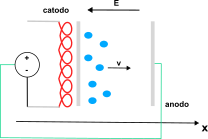
\includegraphics[width=0.4\textwidth]{images/cathodic}  % Include your image here
\end{wrapfigure}

Consideriamo un apparato sperimentale costituito da un tubo sottovuoto al cui interno \`e presente  una lastra di metallo riscaldata da una serpentina metallica e in sua opposizione un ulteriore lastra metallica. Il primo elemento prende il nome $catodo$, mentre il secondo $anodo$. Se generiamo una caduta di tensione tra le due lastre facendo passare al loro interno una corrente elettrica, avremo che tra le due piastre si forma un campo elettrico $\bold{E}$.

 Gli elettroni presenti sul catodo, eccitati dal calore della serpentina, verranno attratti verso l'anodo creando un flusso di corrente per via della forza esercitata su di essi dal campo elettrico generato.
\begin{equation*}
	\bold{F} = -e (-E \hat{u}_{n}) =eE \hat{u}_{n}
\end{equation*}
dove $u_n$ \`e il versore ortogonale al piano. L'accelerazione esercitata sugli elettroni sar\`a data 
\begin{equation*}
	\bold{a} = \frac{eE}{m}\hat{u}_n
\end{equation*}
La legge oraria che descrive il modo degli elettroni \`e dunque data da 
\begin{equation*}
	x = \frac{1}{2}at^2 = \frac{1}{2}\frac{v^2}{a} 
\end{equation*}
e la rispettiva velocit\`a
\begin{equation*}
	v = \sqrt{2ax}
\end{equation*}
Definita $\bold{A}$ l'area della superficie delle lastre metalliche di anodo e catodo, avremo che la densit\`a di corrente \`e data da 
\begin{equation*}
	\bold{J} = nev \hat{u}_n
\end{equation*}
 equindi la corrente \`e pari a 
 \begin{equation*}
 	I = \bold{J} \cdot \bold{A} = \rho \langle v \rangle A 
 \end{equation*}
 che \`e costante nel tempo, ovvero stazionaria. Possiamo dunque desumere che $\rho(x)v(x) = cost $ e quindi 
 \begin{equation*}
 	\rho(x) \sim \frac{1}{\sqrt{x}}
 \end{equation*}
 Le cariche subiranno un addensamento maggiore in prossimit\`a del catodo.
 

 \section{Legge di Amp\`ere}

Introduciamo la prima equazione della magnetostatica,
\begin{equation}
	\nabla \times \bold{B} = \mu_0 \bold{J}
\end{equation}
conosciuta anche come \textit{legge di Amp\`ere} nella sua forma locale. Per dare una definizione pi\`u generale della legge di amp\`ere definiamo la sua forma integrale. Presa una superficie aperta S con contorno $C = \partial S$, integrando (2.3) rispetto a tale superficie passiamo dalla forma differenziale all'integrale di lineare su C,utilizzando il teorema di Stokes 
\begin{equation*}
	\int_{S} (\nabla \times \bold{B})\cdot \bold{dS} = \oint_{C} \bold{B} \cdot \bold{dr} = \mu_0 \int_{S} \bold{J} \cdot \bold{dS}
\end{equation*}
Dove consideriamo il vettore $\bold{S}$ con una direzione ortogonale alla superficie S e con verso uscente. L'integrale di linea lungo il contorno \`e calcolato considerando la regola della mano destra, nel senso che se orientiamo il pollice della mano destra nella direzione $\bold{\hat{n}}$, allora l'indice indica il senso di percorrenza attorno a C dell'integrale di linea.
\newline

L'integrale della densit\`a corrente rispetto alla superficie S \`e equivalente alla corrente I che passa attraverso S, e quindi la legge di amp\`ere in forma integrale \`e data da
\begin{equation}
	\oint_{C} \bold{B} \cdot \bold{dr} = \mu_0 I
\end{equation}

Da un punto di vista applicativo, in generale la legge (2.4) non \`e sufficiente da sola a determinare la forma del campo magnetico, ma \`e necessario utilizzare delle informazioni in pi\`u. Ci sono per\`o alcuni casi in cui utilizzando osservazioni sulla simmetria del problema \`e sufficiente nella determinazione di $\bold{B}$.

Infine si osserva che si \`e ricavata la legge (2.3) ipotizzando che le correnti siano stazionarie. La condizione  $\nabla \cdot \bold{J} = 0$ \`e garantita dalle propriet\`a del rotore dove $\nabla \cdot (\nabla \times \bold{F}) =0 $ per qualsiasi vettore $\bold{F}$.


\subsection{Principio di sovrapposizione per il campo magnetico}
Per una corrente passante attraverso un circuito chiuso, sappiamo per la legge di amp\`ere che 
\begin{equation*}
	\oint_{C} \bold{B} \cdot d\bold{l} = \mu_0 I
\end{equation*}
immaginiamo ora che il cammino $C$ sia attraversato da pi\`u correnti $I_k$, ciascun filo generer\`a un campo magnetico
\begin{equation*}
	\bold{B}_k =\frac{\mu_0 I_k}{2 \pi r_k}\hat{u}_{\theta}
\end{equation*}
per il principio di sovrapposizione il campo magnetico positivo, \`e dato da $\bold{B} = \sum_{k} \bold{B}_k$. La legge di Amp\`ere assume l'esprezzione
\begin{equation*}
	\oint_{C} \bold{B} \cdot d\bold{l} = \sum_{k} \oint_{C} \bold{B}_k \cdot d\bold{l} = \mu_0 \sum_{k}I_k = \mu_0 I_{c}
\end{equation*}
dove $I_c = \sum_k I_k$ e prende il nome di \textit{corrente concatenata}. Se immaginiamo di avere un numero infinito di fili portatori di corrente, avremo che $dI = \bold{J} \cdot d\bold{A}$ e dunque 
\begin{equation}
	\oint_{C} \bold{B} \cdot d \bold{l} = \mu_0 \int dI  = \mu_0 \int \bold{J} \cdot d\bold{A}
\end{equation}
Tale risultato \`e equivalente a considerare l'integrale sulla desit\`a di corrente di tutta la superficie A delimitata da C. Quanto discusso vale solo per correnti stazionarie come nel caso di un solo filo dato che deve valere 
\begin{equation*}
	\nabla \cdot \bold{J} = 0 
\end{equation*}
La relazione (2.5) possiamo interpretarla nel seguente modo:
\begin{center}
	\textit{La circuitazione di $\bold{B}$} lungo un cammino chiuso C \`e equivalente al flusso di $\bold{J}$ attraverso qualsiasi superficie A delimitata dalla curva chiusa C.
\end{center}
\subsection{Filo infinito percorso da una corrente}

Consideriamo un filo di lunghezza infinita in cui scorre una corrente I. Che orientiamo lunga le direzione $\hat{\bold{z}}$. La simmetria del problema suggerisce di usare delle coordinate cilindriche $(r,\varphi,z)$, dove $r = \sqrt{x^2 + z^2}$ \`e il raggio del filo misurato dal suo centro.
%METTERE IMMAGINE DEL FILO INFINITO QUI%
\newline

Consideriamo una superficie aperta S giacente nel piano (x,y), con centro coincidente con quello del filo. Affinch\`e  l'integrale di linea definito in (2.4) non sia nullo, \`e necessario che il campo magnetico abbia delle componenti lungo la circonferenza del disco. Per dimostrarlo ci basta considerare la forma locale della legge di Amp\`ere 
\begin{equation*}
\nabla \times \bold{B} = \mu_0 \bold{J} 
\end{equation*}
dato che la corrente scorre lungo l'asse $\hat{\bold{z}}$ avremo che 
\begin{equation*}
	(\nabla \times \bold{B})_z = \mu_0 J_z \iff  \frac{1}{r} \left(\frac{\partial (rB_{\theta})}{\partial r} - \frac{\partial B_r}{\partial \theta } \right) = \mu_0J_z
\end{equation*}
Per simmetria del problema osserviamo che lungo $\theta$ la componente radiale del campo magnetico \`e costante e quindi 
\begin{equation*}
	\frac{1}{r }\frac{\partial(r B_\theta)}{\partial r} = \left \{ \begin{array}{l}
	\mu_0J_z \quad r \leq R \\
	0 \quad r > R
	\end{array}\right.
\end{equation*}
Risolvendo l'equazione differenziale ordinaria per quadrature abbiamo che 
\begin{equation*}
	B_{\theta} = \left \{ \begin{array}{l}
		\frac{\mu_0 J_z r}{2} + \frac{k_1}{r} \quad r \leq R \\
		\frac{k_2}{r} \quad r > R
	\end{array}\right.
\end{equation*}
Per determinare le costanti d'integrazione, osserviamo che se posizioniamo una carica lungo l'asse $z$ passante per il centro del filo, per simmetria $B_\theta(0) = 0$ e quindi $k_1 =0$. Mentre per $k_2$ imponiamo la continuit\`a del campo sulla superficie del filo, ovvero
\begin{equation*}
	B(R^-) = B(R^+) \iff	 \frac{k_2}{R} = \frac{\mu_0J_zR}{2} \Rightarrow k_2 = \frac{\mu_0I}{2\pi}
\end{equation*} 
per $J = \frac{I}{\pi R^2}$. Possiamo dunque concludere che il campo magnetico del filo \`e dato da 
\begin{equation*}
	B_\theta (r) = \left \{ \begin{array}{l}
		\frac{\mu_0Ir}{2 \pi R^2} \quad r \leq R \\
		\frac{\mu_0I}{2 \pi r} \quad r > R
	\end{array}\right.
\end{equation*}  
\begin{figure}[!ht]
\vspace{0.1in}
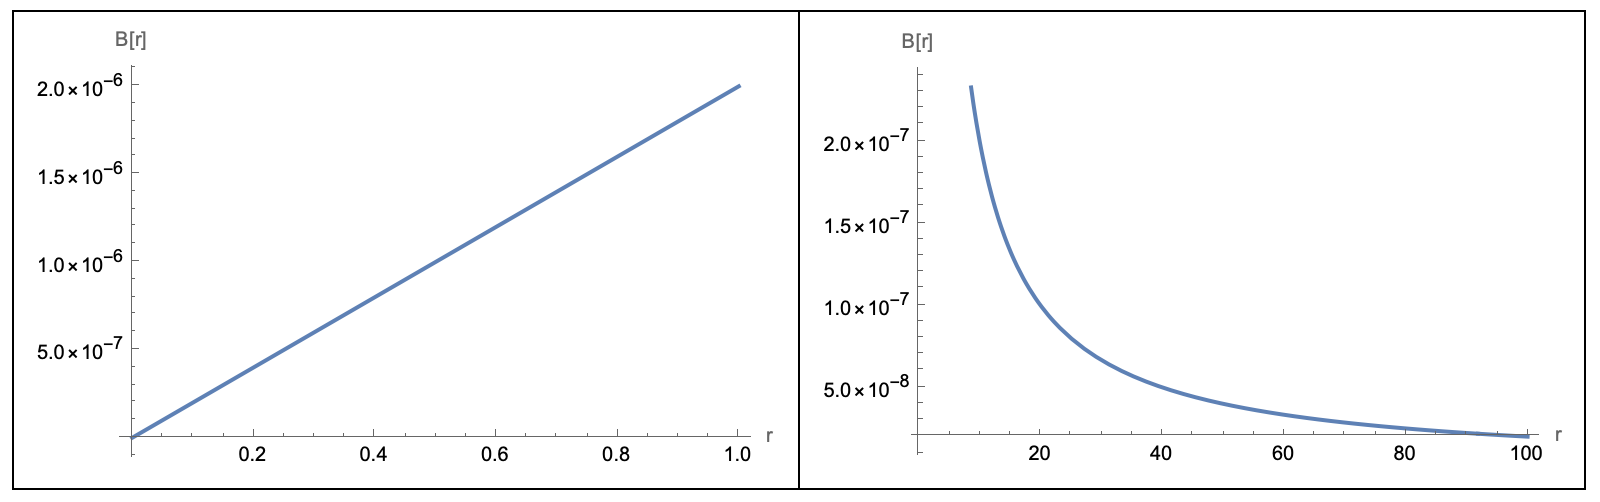
\includegraphics[scale = 0.48]{images/wiremagneticfield}	
\centering
\vspace{0.1in}
\caption{Campo magnetico di un filo di raggio R=1}
\end{figure}

\subsection{Correnti di superficie e discontinuit\`a}

Consideriamo un piano giacente nel piano (x,y), ovvero $z = 0$, sul quale \`e presente un densit\`a di corrente che definiamo $\bold{K}$. Dove con $\bold{K}$ si intende una densit\`a di corrente definita rispetto alle unit\`a d'area. Intuitivamente possiamo pensare ad un piano attraversato da corrente come infinite fili allineati in parallelo.

Consideriamo la corrente con direzione lungo $x$: $\bold{K} = K \hat{\bold{x}}$.
%IMMAGINE PIANO QUI%
\newline

\noindent Affinch\`e $\bold{J} \neq 0$, abbiamo bisogna che l'integrale di linea del campo sia lungo il bordo di una superficie attraverso cui passa la corrente $\bold{K}$. Se vediamo il piano come un numero infinito di fili in parallelo, per simmetria del problema, il campo magnetico pu\`o esistere solo lungo la direzione $y$. 
%IMMAGINE QUI%
Dove $\bold{B}$ ha verso lungo $-\hat{\bold{y}}$ quando $z > 0$ e lungo $\hat{\bold{y}}$ per $z < 0$. Definiamo
\begin{equation*}
	\bold{B} = - B(z) \bold{\hat{y}}
\end{equation*}
dove $B(z)=-B(-z)$. Utilizzando la legge di Amp\`ere su una superficie aperta come in figura:
%IMMAGINE QUI%
con lunghezza L, lungo la direzione $y$ rispetto $\pm z$. Abbiamo che 
\begin{equation*}
	\oint_{C} \bold{B} \cdot \bold{dr} = LB(z) -LB(-z) = 2LB(z) = \mu_0 KL
\end{equation*}
dunque il campo magnetico misurato attorno ad piano attraversato da una corrente di superficie \`e costante e misura:
\begin{equation*}
	B(z) = \frac{\mu_0K}{2} \quad z>0
\end{equation*}
Il risultato ottenuto \`e simile a quanto discusso per una distribuzione di carica planare infinita. Analogamente alla discussione elettrostatica, dove la componente del campo elettrostatico \`e discontinua in direzione ortogonale al piano, per il campo magnetico si ha il medesimo risultato, ma per la componente con  direzione tangenziale alla superficie . Infatti
\begin{equation*}
	B(z \to 0^+) - B(z \to 0^-) = \mu_0K
\end{equation*}
tale risultato \`e valido per qualsiasi corrente di superficie $\bold{K}$. Invece risulta che la componente $\bold{B}_{\perp}$ \`e continua.

\subsection{Flusso del campo magnetico}
Per il campo magnetico vale il seguente risultato:
\begin{center}
\fbox{Il flusso di $\bold{B}$ attraverso una qualunque superficie chiusa \`e nullo.}
\end{center}
che analitacemente esprimiamo nel secondo modo:
\begin{equation*}
	\oint_{S} \bold{B} \cdot \bold{da} = 0 \iff \nabla \cdot \bold{B} =0
\end{equation*}

La relazione $\nabla \cdot \bold{B} = 0$ vale per qualunque distribuzione di sorgenti. Per esempio se consideriamo un elemento come somma di fili, avremo che per il principio di sovrapposizione
\begin{equation*}
	\nabla \cdot \bold{B} = \nabla \cdot \left (\sum_{n} \bold{B}_{n}\right ) = \sum_{n} \nabla \cdot \bold{B}_n =0
\end{equation*}
ottenendo in questo modo un sistema di equazioni differenziali omogenee. Le linee del campo magnetico sono sempre chiuse ( si dice che: "il campo magnetico \`e solenoidale"). Inoltre non esistono sorgenti di monopolo magnetico, il campo magnetico elementare ha sempre forma dipolare (pensate ad una calamita).

\begin{theorem}[Teorema di unicit\`a]
	Il sistema di equazioni differenziali 
	\begin{equation}
		\left \{ \begin{array}{l}
			\nabla \times \bold{B} = \mu_0 \bold{J} \\
			\nabla \cdot \bold{B} = 0
		\end{array}\right.
	\end{equation}
costituito dalle equazioni di Maxxwell, definisce univocamente il campo $\bold{B}$ soluzione, per sorgenti finite, ovvero $B \to 0$ per $r \to \infty$.
\end{theorem}
\begin{proof}
	Siano $B_1$ e $B_2$ due soluzioni del sistema di equazioni (2.5), definiamo
	\begin{equation*}
		\bold{D} = \bold{B}_{1} - \bold{B}_2
	\end{equation*}
che \`e un campo conservativo, dato che 
\begin{equation*}
	\nabla \times \bold{D} = \nabla \times \bold{B}_1 - \nabla \times \bold{B}_2 = \mu_0\bold{J} -\mu_0 \bold{J} =0
\end{equation*}
Essendo il campo $\bold{D}$ irrotazionale, possiamo legarlo ad una funzione scalare $\varphi$ tale per cui $\bold{D} = \nabla \varphi$.

La funzione $\varphi$ soddisfa l'equazione di Laplace 
\begin{equation*}
	\nabla^2 \varphi =0
\end{equation*}
Inoltre sotto l'ipotesi di sorgenti finite avremo che $\varphi(r)|_{r \to \infty} = \varphi_0$ costante, dato che $\bold{D} \to 0 $ per $\bold{r} \to \infty$. In conclusione dato che $\varphi_0$ \`e costante ovunque, si ha che $\bold{D}=0$ e dunque $\bold{B_1} =\bold{B_2}$, dimostrando cos\`i l'unicit\`a della soluzione

\end{proof}

\subsection{Solenoide}

Un solenoide \`e una superficie cilindrica costituita da spire attraversate da una corrente ( in generale non \`e necessario per un solenoide che le spire ti attorciglino ottenendo una forma cilindrica, esistono anche solenoidi toroidali). Per semplicit\`a assumiamo che il cilindro sia infinitamente lungo, in modo da trascurare gli effetti al bordo.
\newline

%IMMAGINE QUI!%

Per un discorso di simmetria della geometria considerata, descriviamo il sistema utilizzando le coordinate cilindriche $(r,\varphi,z)$, con l'asse $\hat{\bold{z}}$ che attraversa il centro del cilindro. Per simmetria, il campo $\bold{B}$ punta lungo l'asse $\hat{\bold{z}}$, per dimostrarlo basta studiare il campo magnetico di una singola spira e applicare il principio di sovrapposizione. L'intensit\`a del campo \`e legata alla distanza radiale $\bold{B} = B(r) \hat{\bold{z}}$. Ogni campo di questo tipo soddisfa la legge di Maxxwell $\nabla \cdot \bold{B} = 0$.
\newline

%IMMAGINE QUI%

Per determinare il valore del campo magnetico consideriamo la forma differenziale della legge di amp\`ere. Ovunque eccetto la superficie del solenoide abbiamo $\bold{J} =0$ e 
	\begin{equation*}
		\nabla \times \bold{B} = 0 \Rightarrow \frac{dB}{dr} = 0 \Rightarrow B(r) = costante
	\end{equation*} 
Al di fuori del solenoide per il teorema di unicit\`a sappiamo che deve valere $B(r) \to 0$ per $r \to \infty $ e B(r) \`e costante. Per determinare il campo magnetico all'interno del solenoide utilizziamo la forma integrale della legge di Amp\`ere e consideriamo una superficie S aperte, il cui contorno \`e dato da una curva chiusa C come in figura. Abbiamo che 
\begin{equation}
	\oint \bold{B} \cdot \bold{dr} = B_z(0)L
\end{equation} 
Per determinare il valore di $B_z(0)$ consideriamo un porzione infinitesima $dz$ del cilindro percorso dalle spire e quindi attraversato da una corrente $dI$. Definiamo la grandezza $n = N/ L$ che definisce il numero di spire per unit\`a di lunghezza. La corrente attraversata dalla porzione dz sar\`a data da 
\begin{equation*}
	dI = nidz
\end{equation*}
Data la forma cilindra, la porzione dz geometricamente coincide con quella di un anello di altezza $dz$, dunque possiamo calcolare il suo campo magnetico per un punto lungo l'asse $\bold{\hat{z}}$ fissato a distanza $\bold{r}$ dal suo bordo.
\begin{equation*}
	dB = \frac{\mu_0}{2}\frac{b^2}{r^3}dI = \frac{\mu_0}{2}ni \frac{b^2}{r^2}\frac{dz}{r} = \frac{\mu_0}{2}dz\sin\theta = dB_z
\end{equation*}
%IMMAGINE QUI%
integrando i contributi infinitesimi abbiamo che 
\begin{equation*}
	B_z =  \frac{\mu_0}{2}ni \int_{\theta_1}^{\theta_2}\sin \theta d\theta = \frac{\mu_0}{2}ni[\cos\theta_1-\cos\theta_2]
\end{equation*}

Preso $\theta_1 = 0$ e $\theta_2 = \pi$ abbiamo che 
\begin{equation*}
	B_z(0) = \mu_0 ni
\end{equation*}
dunque il campo all'interno del solenoide recuperando l'equazione (2.6) \`e 
\begin{equation*}
	B_z(0)L = \mu_0niL
\end{equation*}
coincide proprio con $B_z(0)$. Inoltre passando dal bordo interno a quello esterno di ha una discontinuit\`a del campo $\Delta_{//} = \mu_0ni$. Notare che definita $K = IN$, quando trovato \`e consistente con l'equazione generale trovata per la discontinuit\`a del campo magnetico dovuto a una corrente di superficie.


\section{Potenziale vettore}

Per le distribuzioni corrente viste fino a questo momento, le argomentazioni sulla simmetria sono sufficienti per determinare un campo mangnetico che soddisfi la condizione 
\begin{equation*}
	\nabla \cdot \bold{B} = 0
\end{equation*}
Per discutere di correnti pi\`u generiche, questo non \`e pi\`u sufficiente. Per farlo partiamo dalla seguente osservazione: sappiamo che per un vettore generico $\bold{A}$, vale la propriet\`a 
\begin{equation*}
	\nabla \cdot (\nabla \times \bold{A}) =0
\end{equation*}
dunque se troviamo un vettore $\bold{A}$ rispetto a cui il campo $\bold{B}$ pu\`o essere scritto come suo rotore
\begin{equation*}
	\bold{B} = \nabla \times \bold{A}
\end{equation*}
in automatico abbiamo soddisfatto l'equazione di Maxxwell $\nabla \cdot \bold{B} = 0$. Il vettore $\bold{A}$ che soddisfa questo tipo di relazione prende il nome di \textit{potenziale vettore}. Sostituendo nella legge di amp\`ere in forma differenziale, questa diventa
\begin{equation}
	\nabla \times \bold{B} = - \nabla^2\bold{A} + \nabla(\nabla \cdot \bold{A}) = \mu_0 \bold{J}
\end{equation}
Risolvendo questa equazione per $\bold{A}$ determiniamo anche il campo $\bold{B}$.

\subsection{Monopoli Magnetici}

Nei paragrafi precedenti abbiamo dimostrato analiticamente l'equazione di Maxxwell $\nabla \cdot \bold{B} = 0 $, ma non ci siamo mai soffermati nel discuterne il significato fisico. La sua interpretazione \`e molto semplice, infatti ci dice che nei punti considerati non \`e presente carica magnetica. Se esistesse una sorgente puntiforme di carica magnetica $g$, per un campo magnetico $\bold{B}$ e che decresce quadraticamente rispetto alla distanza radiale, avremmo 
\begin{equation*}
	\bold{B} = \frac{g}{4\pi r^2}\hat{u}_{r}
\end{equation*} 
Un oggetto di questo tipo viene di solito chiamato \textit{monopolo magnetico}. Le equazioni di Maxxwell della magnetostatica ci dicono che oggetti di questo tipo non esistono, inoltre in natura non sono trovate evidenze sperimentali che ne dimostrino l'esistenza.
\newline

\noindent Ma siamo davvero sicuri che i monopoli magnetici non esistono?   Per esempio se  adattassimo le equazioni di Maxwell, permettendo la presenza di carica magnetica, scrivendo
\begin{equation*}
	\nabla \cdot \bold{B} = \rho_m
\end{equation*}
per $\rho_m$ distribuzione di carica magnetica, avremmo che non possiamo pi\`u usare il vettore potenziale $\bold{A}$, ma \`e davvero una cos\`i grande perdita?
\newline

I problemi insorgono quando iniziamo a considerare la meccanica quantistica, dove siamo obbligati ad utilizzare il potenziale vettore $\bold{A}$. Non sono l'intera trattazione dell'elettromagnetismo in meccanica quantistica \`e basato sull'uso di $\bold{A}$, ma ci sono addirittura esperimenti che rilevano certe propriet\`a di $\bold{A}$ e che vengono persi quando calcoliamo $\bold{B} = \nabla \times \bold{A}$, come nel caso dell'effetto Aharanov-Bohm (argomento trattato nel corso di struttura della materia al terzo anno).

Possiamo riassumere quanto discusso osservando che buona parte della teoria e della realt\`a sperimentale sia consistente nell'asserire la non esistenza dei monopoli magnetici... e invece no! ci sono buone argomentazioni che lasciano pensare all'esistenza di questi oggetti esotici. Dirac  ha dimostrato che \`e possibile introdurre un vettore potenziale $\bold{A}$ che permette di avere carica magnetica, ma solo se questa carica $g$, ma solo se la quantit\`a di carica \`e legata a quella di un elettrone $e$, mediante la relazione 
\begin{equation*}
	ge = 2 \pi \hbar n \quad n \in \mathbb{Z}
\end{equation*}
Questa equazione prende il nome di \textit{condizione di quantizzazione di Dirac}.

\subsection{Trasformazioni di Gauge}

La scelta di $\bold{A}$ nell'equazione (2.7) \`e tutt'altro che univoca: ci sono diversi potenziali vettore che descrivono il medesimo campo magnetico $\bold{B}$. Questo \`e dovuto al fatto che il rotore del gradiente \`e automaticamente nullo. Questo vuol dire che possiamo aggiungere ad $\bold{A}$ un qualsiasi vettore potenziale della forma $\nabla_{\chi}$ per una cerca funzione $\chi$ e il campo magnetico resta sempre lo stesso,
\begin{equation*}
	\bold{A}' = \bold{A} + \nabla_{\chi} \Rightarrow \nabla \times \bold{A}' = \nabla \times \bold{A}
\end{equation*}
Una trasformazione di questo tipo su $\bold{A}$ prende il nome di \textit{trasformazione di gauge}. Scegliendo in modo intelligente $\chi$, riusciamo a semplificare i conti per determinare il campo magnetico.

\begin{theorem}[Coulomb gauge]
	\`E sempre possibile trovare una trasformazione di gauge $\chi$ tale che $\bold{A}'$ soddisfi $\nabla \cdot \bold{A}' = 0$. Si fa riferimento a una scelta di questo tipo come \textit{Coulomb gauge}.
\end{theorem}

\begin{proof}
	Supponiamo di conoscere a priori un potenziale vettore $\bold{A}$ tale per cui $\bold{B} = \nabla \times \bold{A}$, ma quando calcoliamo la divergenza otteniamo un espressione $\nabla \cdot \bold{A} = \psi(\bold{x})$. Se invece scegliamo $\bold{A}' = \bold{A} + \nabla_{\chi}$, avremo che la sua divergenza \`e data da 
	\begin{equation*}
		\nabla \cdot \bold{A}' = \nabla \cdot \bold{A} + \nabla^2_{\chi} = \psi(\bold{x}) + \nabla^2_{\chi}
	\end{equation*}
Dunque se vogliamo avere $\nabla \cdot \bold{A}' = 0 $, basta che prendiamo una trasformazione di gauge $\chi$ per cui
\begin{equation*}
	\nabla^2_{\chi} = -\psi(\bold{x})
\end{equation*}
ma questa non \`e altro che l'equazione di Poisson. Per quanto discusso nel capitolo di elettrostatica sappiamo sempre che questa equazione ammette sempre soluzione.

\end{proof}

\newpage 

\subsection{Legge di Biot-Savart}

Utilizziamo ora il potenziale vettore per determinare il campo magnetico $\bold{B}$ generato da una distribuzione di corrente generica. Assumiamo che stiamo usando con un gauge di Coulomb e che sia soddisfatta la condizione $\nabla \cdot \bold{A} =0 $ per il potenziale vettore $\bold{A}$. La legge di amp\`ere definita in (2.7) diventa molto pi\`u semplice da risolvere
\begin{equation}
	\nabla^2 \bold{A} = - \mu_0 \bold{J}
\end{equation}
che \`e equivalente a risolvere il sistema di equazioni di Poisson 
\begin{equation*}
	\nabla^2 A_i = -\mu_0J_i \quad (i=1,2,3)
\end{equation*}
Considerando la risoluzione delle singole equazioni rispetto ad un sistema di coordinate cartesiane, la soluzione delle equazioni \`e identica a quella ottenuta nella discussione elettrostatica. Ottenendo
\begin{equation*}
	A_i(\bold{x}) = \frac{\mu_0}{4 \pi} \int_{V} d^3\bold{x}' \; \frac{J_i(\bold{x}')}{|\bold{x}-\bold{x}'|} \quad (i =1,2,3)
\end{equation*}
che in notazione vettoriale diventa
\begin{equation}
	\bold{A}(\bold{x}) = \frac{\mu_0}{4 \pi} \int_{V} d^3\bold{x}' \; \frac{\bold{J}(\bold{x}')}{|\bold{x} - \bold{x}'|}
\end{equation}
Vogliamo ora verificare che (2.9) sia una soluzione univoca dell'equazione di Amp\`ere definita in (2.7), questo \`e vero se il risultato $\bold{A}$ soddisfa la condizione di gauge di Coulomb data da $\nabla \cdot \bold{A} =0$. Dunque andando a calcolare la divergenza di $\bold{A}$ abbiamo che
\begin{equation*}
	\nabla \cdot \bold{A}(\bold{x}) = \frac{\mu_0}{4\pi} \int_{V} d^3\bold{x}' \; \nabla \cdot \left ( \frac{\bold{J}(\bold{x}')}{|\bold{x}-\bold{x}'|}\right)
\end{equation*}
dove gli indici di $\nabla$ coincidono con quelli di $\bold{J}$, ma l'operatore $\nabla$ agisce su $\bold{x}$ non su $\bold{x}'$. Preso atto di questa considerazione, possiamo scrivere l'equazione nel seguente modo
\newpage 
\begin{align*}
	\nabla \cdot \bold{A}(x) & = \frac{\mu_0}{4 \pi} \int_{V} d^3\bold{x}' \; \bold{J}(\bold{x}') \cdot \nabla \left( \frac{1}{|\bold{x} -\bold{x}'|} \right)\\[0.5cm]
	& = - \frac{\mu_0}{4\pi} \int_V d^3\bold{x}' \; \bold{J}(\bold{x}') \cdot \nabla' \left( \frac{1}{|\bold{x} -\bold{x}'|} \right) 
\end{align*}
Dove $\nabla'$ differenzia rispetto a $\bold{x}'$. Per ottenere tale risultato, si \`e usato il fato che se si differenzia $1/|\bold{x} - \bold{x}'|$ rispetto ad $\bold{x}$, si ottiene il medesimo risultano a differenza di un segno meno differenziando rispetto a $\bold{x}'$. Dato che $\nabla'$ \`e all'interno dell'integrale e $\bold{J}(\bold{x}')$ dovremmo derivare per parti. Ottenendo 
\begin{equation*}
\nabla \cdot \mathbf{A}(\mathbf{x})=-\frac{\mu_0}{4 \pi} \int_V d^3 x^{\prime}\left[\nabla^{\prime} \cdot\left(\frac{\mathbf{J}\left(\mathbf{x}^{\prime}\right)}{\left|\mathbf{x}-\mathbf{x}^{\prime}\right|}\right)-\nabla^{\prime} \cdot \mathbf{J}\left(\mathbf{x}^{\prime}\right)\left(\frac{1}{\left|\mathbf{x}-\mathbf{x}^{\prime}\right|}\right)\right]
\end{equation*}
Il secondo termine scompare perch\`e per ipotesi stiamo considerando correnti stazionarie per cui $\nabla' \cdot \bold{J} = 0$. Il primo termine risulta essere nullo se consideriamo regioni di spazio in cui $\bold{J}(\bold{x}) = 0$, assumendo che questo sia al caso possiamo concludere che 
\begin{equation*}
	\nabla \cdot \bold{A} = 0
\end{equation*}
e quindi l'univocit\`a della soluzione per l'equazione (2.7).
\newpage 


\subsubsection{Campo magnetico}

Dalla soluzione (2.9) possiamo determinare il campo magnetico per $\bold{B} = \nabla \times \bold{A}$, ricordando che $\nabla$ agisce su $\bold{x}$ e non su $\bold{x}'$. Consideriamo un tratto $dl$ infinitesimo di un generico filo a cui possiamo associare un contributo infinitesimo al potenziale vettore 
\begin{equation*}
	d\bold{A} = \frac{\mu_0I}{4\pi} \frac{1}{r} d\bold{\hat{l}}
\end{equation*}

Il contributo infinitesimo al campo magnetico \`e dato da 
\begin{align*}
	d\bold{B} & = \nabla \times \bold{dA} = \frac{\mu_0I}{4 \pi } \; \nabla \times \left( \frac{d \bold{\hat{l}}}{r}\right)= \\[0.5cm]
	& = \frac{\mu_0 I}{4 \pi} \left [ \nabla \left( \frac{1}{r}\right) \times d\bold{\hat{l}} + \frac{1}{r} \nabla \times d\bold{\hat{l}}\right] = - \frac{\mu_0 I}{4 \pi} \; \frac{\hat{u}_{r} \times d\bold{\hat{l}}}{r^2} = \frac{\mu_0 I}{4 \pi} \; \frac{d \bold{\hat{l}} \times \hat{u}_r}{r^2}
\end{align*}
dove secondo addendo della somma risulta essere nullo perch\`e $d\bold{\hat{l}}$ \`e costante. Ora che abbiamo legato il campo magnetico alla corrente, possiamo definire 
\begin{equation}
	\bold{B}(\bold{x}) = \frac{\mu_0I}{4\pi} \oint_{C} \frac{d \bold{\hat{l}} \times \hat{u}_r}{r^2} = \frac{\mu_0I}{4\pi} \oint_{C} \frac{d \bold{\hat{l}} \times \hat{u}_r}{|\bold{r} -\bold{r}'|^2}
\end{equation}
tale risultato prende il nome di \textit{legge di Biot-Savart}. Per ottenere l'espressione rispetto l'intensit\`a di corrente abbiamo riscritto la densit\`a di corrente in un volume come 
\begin{equation*}
	\bold{J}(\bold{x}')dV = JA \;d\bold{\hat{l}} = Id\bold{\hat{l}}
\end{equation*}
dove A \`e la sezione del filo e la direzione $d \bold{\hat{l}}$ \`e tangente a C, che coincide con la curva formata dal filo.

\subsubsection{Esempio: Filo infinito rivisitato}
%IMMAGINE QUI%
Dato un sistema in cui \`e presente un filo infinito attraversato da una corrente, vogliamo verificare che sia verificata la legge di Biot-Savart. Passando in coordinate cilindriche, consideriamo un punto lungo sull'asse $\hat{\bold{z}}$ passante per il centro del filo e definiamo $r^2 = x^2 + y^2$ come coordinata radiale. L'elemento di filo \`e parametrizzato come $d\hat{\bold{x}} = \hat{\bold{z}}dz$ e per un punto $\bold{x}$ distante dal filo, il vettore $d\bold{x}' \times (\bold{x}- \bold{x}')$ \`e tangente alla circonferenza di raggio $r$ attraverso cui passa la corrente con intensit\`a I,
\begin{equation*}
	d\bold{x}' \times (\bold{x} -\bold{x}') = r dz \;\hat{u}_{\varphi} 
\end{equation*}
dunque avremo 
\begin{equation*}
	\bold{B} = \frac{\mu_0I}{4\pi} \int_{\mathbb{R}} dz \; \frac{r}{(r^2+z^2)^{3/2}} = \frac{\mu_0I}{2 \pi r} \hat{u}_{\varphi}
\end{equation*}
ritrovando lo stesso risultato per la legge di Amp\`ere.

\section{Dipoli magnetici}

Abbiamo visto che le equazioni di Maxwell non permettono l'esistenza di monopoli magnetici e che il l'intensit\`a del campo magnetico $B \sim 1/r^2$. In generale come decade il campo magnetico dovuto a distribuzioni di corrente localizzate in una regione di spazio? Nei prossimi paragrafi vedremo che se si \`e sufficientemente lontani dalla corrente, il campo appare come quello generato da un dipolo magnetico.

\subsection{Corrente in una spira circolare}

%IMMAGINE QUI%

Consideriamo una spira circolare C con raggio R attraversata da una corrente con intensit\`a I. Per calcolare il campo magnetico lontano dalla spira, utilizziamo l'espressione originale che abbiamo ottenuto per il potenziale vettore $\bold{A}$.
\begin{equation*}
	\bold{A}(\bold{r}) = \frac{\mu_0}{4 \pi} \int_{V} d^3r' \; \frac{\bold{J}(\bold{r}')}{|\bold{r}-\bold{r}'|}
\end{equation*}
In termini della corrente il vettore potenziale diventa
\begin{equation*}
	\bold{A}(\bold{r}) = \frac{\mu_0 I}{4 \pi} \oint_{C} \frac{d\bold{r}'}{|\bold{r}-\bold{r}'|}
\end{equation*}
Siccome stiamo calcolando il campo in un punto $\bold{r}$ molto lontano dalla corrente, avremo che l'argomento dell'integrale pu\`o essere espanso con Taylor 
\begin{equation*}
	\frac{1}{|\bold{r} - \bold{r}'|} = \frac{1}{r} + \frac{\bold{r} \cdot \bold{r}'}{r^3}+...
\end{equation*}
e quindi abbiamo
\begin{equation*}
	\bold{A}(\bold{r}) = \frac{\mu_0 I}{4 \pi} \oint_{C} d\bold{r}' \; \left ( \frac{1}{r} + \frac{\bold{r} \cdot \bold{r}'}{r^3}+...\right)
\end{equation*}
Il primo termine dell'espansione \`e nullo perch\`e stiamo integrando lungo un circuito chiuso. Per il secondo termine, lo riscriviamo in una forma pi\`u maneggevole, introducendo il vettore costante $\bold{g}$
\begin{equation*}
	\oint_{C}d\bold{r}' \cdot \bold{g}(\bold{r} \cdot \bold{r}')
\end{equation*}
Osservare che rispetto all'integrale sia $\bold{g}$ che $\bold{r}$ sono vettori costanti. Utilizzando il teorema di Stokes  abbiamo che 
\begin{equation*}
	\oint_{C}d\bold{r}' \cdot \bold{g}(\bold{r} \cdot \bold{r}') = \int_{S} d\bold{S} \cdot \nabla \times (\bold{g}(\bold{r}\cdot \bold{r}')) = \int_{S} dS_i \; \varepsilon_{ijk}\partial_j'(g_kr_lr_l') = \bold{g} \cdot \int_{S} d\bold{S} \times \bold{r}
\end{equation*}
Tale identi\`a \`e verigicata per ogni vettore costante $\bold{g}$, il che vuol dire che deve valere anche per ogni uguaglianza tra vettori e quindi
\begin{equation*}
	\oint_{C}d\bold{r}' \; (\bold{r} \cdot \bold{r}') = \mathcal{S} \times \bold{r}
\end{equation*}
dove $\mathcal{S}$ \`e vettore d'area della superficie S delimitata dalla curva C, dove 
\begin{equation*}
	\mathcal{S} = \int_{S}d\bold{S}
\end{equation*}
Se il circuito C \`e contenuto in un piano, come nel nostro caso, allora il vettore $\mathcal{S}$ \`e ortogonale alla superficie e verso uscente.

Sostituendo nell'espressione del vettore potenziale avremo che 
\begin{equation*}
	\bold{A}(\bold{r}) = \frac{\mu_0}{4 \pi} \frac{\mathcal{S} \times I\bold{r}}{r^3} = \frac{\mu_0}{4 \pi} \frac{\bold{m}\times \bold{r}}{r^3}
\end{equation*}
dove il termine 
\begin{equation}
	\bold{m} = I \mathcal{S} 
\end{equation}
prende il nome di \textit{momento di dipolo magnetico}. Per calcolare il campo magnetico ricordiamo che $\bold{B} = \nabla \times \bold{A}$, e svolgendo i dovuti calcoli algebrici abbiamo che
\begin{equation*}
	\bold{B}(\bold{r}) = \frac{\mu_0}{4 \pi} \left ( \frac{3(\bold{m} \cdot \bold{\hat{r}})\bold{\hat{r}} - \bold{m}}{r^3}\right)
\end{equation*}
che coincide con l'espressione del campo di un dipolo elettrico. In conclusione, per grandi distanza il campo magnetico $\bold{B}$ e $\bold{E}$ risultando essere identici avendo la forma di dipolo.

\subsection{Distribuzione generiche di corrente}
%IMMAGINE QUI%
Consideriamo un circuito generico C chiuso e attraversato da una corrente d'intensit\`a I, giacente nel piano (x,y). Immaginiamo di suddividere il generico circuito in spire quadrate chiuse di lato $b$, in questo modo il campo magnetico complessivo pu\`o essere visto come la somma dei contributi dati dal campo delle singole spire. 

Le correnti di ogni singola spira si cancellano con quelle adiacenti, in questo modo si ha che il contributo \`e dato solo da quella corrente che percorre il circuito C, lasciando cos\`i inalterato il sistema iniziale. Il potenziale vettore \`e dato da 
\begin{equation*}
	\bold{A} = - \frac{\mu_0 }{4 \pi }INb^2\frac{\sin \alpha}{r^2} \hat{u}_x
\end{equation*}
dove il termine $a = Nb^2$ \`e l'area complessiva del circuito, data dal contributo dell'area di N spire quadrate. Posto il momento di dipolo magnetico $\bold{m} = Ia\hat{u}_z$ avremo che il potenziale vettore \`e dato da 
\begin{equation*}
	\bold{A} = \frac{\mu_0}{4\pi} \frac{\bold{m} \times \hat{u}_r}{r^2}
\end{equation*}
Notare che i calcoli svolti sono approssimativi, in quanto se C \`e una curva generica, le spire in prossimit\`a del bordo non avranno dei lati formati da linee rette e dunque non saranno quadrate, e quindi la loro area non \`e $b^2$, ma un qualcosa di pi\`u piccolo. Dunque a seconda di come si sceglie di contare il numero di spire il termine $\bold{m}$ avr\`a un valore diverso, dandone cos\`i una definizione non univoca. Il modo migliore per definire $\bold{m}$ \`e dato dai passaggi usati nel paragrafo precedente. 

\section{Esempi di campi magnetici}

\subsection{Campo magnetico di una spira circolare}

%IMMAGINE QUI%

Dato l'asse $\hat{\bold{z}}$ passante per il centro della spira circolare di raggio $b$ e giacente nel piano (x,y), determiniamo il campo magnetico in un punto lungo $\hat{\bold{z}}$. Per la simmetria dell'anello rimane solo un contributo assiale del campo magnetico per un tratto infinitesimo della spira e utilizzando la legge di Biot-Savart definiamo 
\begin{equation*}
	dB_z = \frac{\mu_0I}{4 \pi} \frac{|d\bold{l} \times \hat{u}_{r}|}{r^2}\cos\theta   = \frac{\mu_0I}{4 \pi} \frac{dl}{r^2}\cos\theta  = \frac{\mu_0I}{4 \pi} \frac{b}{r^3}dl
\end{equation*} 
Procedendo per integrazione 
\begin{equation*}
	B_z(r) = \frac{\mu_0I}{4 \pi} \frac{b}{r^3} \oint_{C}dl = \frac{\mu_0I}{4 \pi} \frac{b}{r^3} \int_{0}^{2\pi} bd\theta = \frac{\mu_0Ib^2}{2} \frac{1}{r^3}
\end{equation*}

%manca la parte sulle linee di campo%

\subsection{Campo magnetico di un solenoide toroidale}

%IMMAGINE QUI%

Dato un solenoide toroidale con angolo minore $a$ e angolo maggiore $b$ attraversato da una corrente I, abbiamo che il campo magnetico ha solo componente angolare 
\begin{equation*}
	\bold{B} = B_\theta \hat{u}_{\theta}
\end{equation*}
questo \`e dovuto al fatto che prese due spire diametralmente opposte, cambia il senso di percorrenza della corrente viaggiando in modo opposto e quindi i campi lungo $u_z$ e $u_r$ sono opposti e di eguale intensit\`a elidendosi in ogni punto per la simmetria dell'oggetto. Per determinare la forma esplicita del campo, definitiamo un circuito di Amp\`ere che racchiuda il toroide, $d\bold{l} = r d\theta \hat{u}_{\theta}$,
\begin{equation*}
	\oint_C \bold{B} \cdot d\bold{l} = \int_{0}^{2\pi} B_\theta r d\theta = B_\theta 2\pi = \left \{ \begin{array}{l}
		0 \quad r<a \; o \; r>b\\
		\mu_0IN \quad \text{altrimenti}
	\end{array}\right.
\end{equation*}
dove N \`e il numero di avvolgimenti del filo conduttore attorno al toroide. Quindi possiamo concludere che 
\begin{equation*}
	B_{\theta}(r) = \left \{ \begin{array}{l}
		0 \quad r \not\in [a,b]\\[0.3cm]
		\frac{\mu_0 N I}{2 \pi r} \quad r \in [a,b]
	\end{array}\right.
\end{equation*}

\section{Forza magnetica}

Abbiamo visto che una corrente produce un campo magnetica, ma una corrente altro non \`e che cariche in movimento. Per una carica $q$ in movimento con velocit\`a $\bold{v}$, questa sar\`a soggetta ad una forza 
\begin{equation*}
	\bold{F} = q\bold{v} \times \bold{B}
\end{equation*}
che prende il nome di \textit{forza di Lorentz}. Questo vuol dire che che se posizioniamo una corrente in prossimit\`a della prima, queste eserciteranno una forza l'una sull'altra.

Dalla forma della forza di Lorentz deduciamo che questa  \`e ortogonale al piano formato dai vettori $\bold{v}$ e $\bold{B}$, e quindi ai suoi singoli vettori. Possiamo desumere che l'accelerazione a cui \`e soggetta la carica sia di natura centripeta 
\begin{equation*}
	\bold{a} = \frac{qvb}{m}
\end{equation*}
Consideriamo una quantit\`a di carica $dq$ passante all'interno di un filo la forza esercitata sulle cariche \`in movimento \`e data da 
\begin{equation*}
	d\bold{F} = dq\bold{v} \times \bold{B} = \frac{dq}{dt}d\bold{l} \times \bold{B} = Id \bold{l} \times \bold{B}
\end{equation*}
che risulta essere consistenza con il risultato empirico ottenuto da Laplace. Dato che le cariche sono vincolate nel filo, e queste subiscono una forza che cerca di portale al di fuori, questo reagisce con una reazione vincolare, esercitando una forza uguale e contraria.

Per velocit\`a ordinare, quindi non relativistiche la forza magnetica \`e molto meno intensa di quella elettrostatica.

\subsubsection{Esempio}

%IMMAGINE QUI%

Consideriamo una distribuzione di carica lineica positiva, il campo generato dalla distribuzione delle cariche \`e dato da 
\begin{equation*}
	\bold{E} = \frac{\lambda }{2 \pi \varepsilon_0}\frac{1}{r} \hat{u}_{r}
\end{equation*}
la forza a cui \`e soggetta una carica esploratrice \`e data da 
\begin{equation*}
	\bold{F}_{E} = q\bold{E} = \frac{q\lambda}{2 \pi \varepsilon_0}\frac{1}{r}\;\hat{u}_{r}
\end{equation*}
Ora invece prendiamo un filo al cui interno scorre della carica q, il campo magnetico sar\`a dato da 
\begin{equation*}
	\bold{B} = \mu_0 \frac{\lambda v}{2 \pi r}\hat{u}_{\theta}
\end{equation*}
e la forza magnetica a cui sono sottoposte le cariche \`e data dalla Forza di Lorentz
\begin{equation*}
	\bold{F}_{B} = q \bold{v} \times \bold{B} = qvB \hat{u}_{r}
\end{equation*}
Mettendo a confronto il modulo delle forze abbiamo che 
\begin{equation*}
	\frac{\bold{F}_B}{\bold{F}_E} = \frac{qvB}{qE} = \mu_0 \varepsilon_0 v^2 = \left (\frac{v}{c}\right)^2\approx 0
\end{equation*}
dove abbiamo posto $c = 1/\sqrt{\varepsilon_0\mu_0}$. Dunque a velocit\`a ordinarie la forza di Coulomb \`e molto pi\`u grande di quella  magnetica.

\subsection{Forza tra due fili}

Abbiamo visto come la forza magnetica porti a deviare le cariche all'interno di un filo e che mantengono la loro direzione di flusso per via della reazione vincolare esercitata dalla struttura. Che cosa succede se facciamo interagire due fili attraversati da corrente ?
\newline

%IMMAGINE QUI%
\noindent Prendiamo due fili in parallelo a distanza $d$ e rispettivamente attraversati da una corrente $I_1$ e $I_2$. La corrente nel primo filo genera un campo magnetico, di conseguenza se le cariche nel secondo filo si muovono con una velocit\`a $\bold{v}$, saranno soggette ad una forza 
\begin{equation*}
	\bold{F} = q \bold{v} \times \bold{B} = q \bold{v} \times \left ( \frac{\mu_0I_1}{2 \pi d}\right)\hat{u}_y
\end{equation*} 
dove $\hat{u}_y$ \`e la direzione del campo magnetico a cui le cariche del secondo filo sono sottoposte. Vogliamo scrivere la velocit\`a $\bold{v}$ in termini della corrente $\bold{I}_2$ del secondo filo. Se abbiamo una densit\`a di particelle $n$ di cui ciascuna trasporta una carica $q$, la densit\`a di corrente sar\`a data da
\begin{equation*}
	\bold{J}_2 = nq \bold{v}
\end{equation*}
Per un filo di sezione A, la corrente \`e data da $I_2 = J_2A$. Per il nostro sistema avremo che $\bold{J_2} = J_2 \hat{u}_{z}$. Calcoliamo la forza esercitata sul filo per unit\`a di lunghezza, $\bold{f}$. Dato che il numero di cariche per unit\`a di lunghezza \`e dato da $nA$ e $\bold{F}$ \`e la forza applicata su ogni carica, abbiamo che
\begin{equation}
	\bold{f} =nA\bold{F} = \left ( \frac{\mu_0 I_1 I_2}{2 \pi d}\right)\hat{\bold{z}} \times \bold{\hat{y}} = - \left ( \frac{\mu_0 I_1 I_2}{2 \pi d}\right) \bold{\hat{x}}
\end{equation}

Se le due correnti hanno la stessa direzione, $I_1 I_2 > 0$,  e quindi la forza tra i due fili \`e attrattiva. Per correnti di segno opposto $I_1 I_2 < 0$ la forza \`e repulsiva.

\section{Cariche in movimento in un campo magnetico uniforme}

Se una particella di massa $m$ si muove lungo una circonferenza di raggio $R$ con velocit\`a costante $v$, su di essa agisce una forza radiale di intensit\`a $F = mv^2/r$, che punto sempre verso il centro ed \`e perpendicolare alla velocit\`a della particella.
\newline

\noindent Nelle sezioni precedenti abbiamo visto come la forza $\bold{F}_{B}$ punti sempre in direzione perpendicolare alla velocit\`a $\bold{v}$ della particella carica e del campo magnetico $\bold{B}$. Siccome, la forza magnetica $\bold{F}_B$ non compie lavoro, l'unica cosa che pu\`o altera \`e la direzione di $\bold{v}$ e non la sua intensit\`a.

In questa sezione cerchiamo di dare una risposta alla domanda: come evolve la dinamica di una particella carica con velocit\`a $\bold{v}$ che interagisce con una campo magnetico uniforme $\bold{B}$?

Ipotizziamo che la particella abbia una carica positiva $+q$ e che la direzione del campo $\bold{B}$ sia entrante nella pagina, inoltre $\bold{v} \perp \bold{B}$ quando si immette nel campo. Sulla particella agir\`a la forza di Lorentz 
\begin{equation}
	\bold{F}_{B} = q\bold{v} \times \bold{B} = -qvB \;\hat{u}_{r}
\end{equation}
troviamo quindi che sulla carica agisce una forza di natura radiale e quindi $\bold{F}_{B}$ \`e una forza di natura centripeta, che porta $q$ a muoversi in senso antiorario lungo un cammino circolare.

%IMMAGINE QUI%

Data l'identi\`a 
\begin{equation*}
	qvB = \frac{mv^2}{r}
\end{equation*}
possiamo determinare il raggio della circonferenza percorsa dalla particella, ottenendo
\begin{equation*}
	r = \frac{mv}{qB}
\end{equation*}
Il periodo $T$ con cui la carica compie una rivoluzione completa \`e dato da 
\begin{equation*}
	T = \frac{2 \pi r}{v} = \frac{2\pi}{v} \frac{mv}{qB} = \frac{2\pi m}{qB}
\end{equation*}
Similmente, la velocit\`a angolare (o frequenza ciclotronica) $\omega$ della particela si deriva calcolando
\begin{equation*}
	\omega = 2 \pi f = \frac{v}{r} = \frac{qB}{m}
\end{equation*}
Se la velocit\`a iniziale della particella carica possiede anche una componente parallela al campo magnetico $\bold{B}$, anzich\`e avere un moto circolare, la traiettoria risultante sar\`a elicoidale 

%IMMAGINE QUI%

In particolare la posizione della particella sar\`a descritta dalle equazioni
\begin{equation*}
	\bold{r}(t) = \left \{ \begin{array}{l}
		x(t) = R\cos(\omega t + \varphi)\\
		y(t) = R\sin(\omega t + \varphi)\\
		z(t) = v_{\parallel} t + z_0
	\end{array}\right.
\end{equation*}
Il passo dell'elica \`e dato da $p = v_{\parallel}T$ dove T coincide con il periodo con cui viene completato un giro nella proiezione sul piano.

\subsection{Moto Cicloidale}

Prendiamo un sistema in cui \`e presente sia un campo elettrico $\bold{E}$ che un campo magnetico $\bold{B}$. Se il campo elettrico possiede solo una componente parallela al campo magnetico che ha direzione lungo $\hat{\bold{z}}$, il moto risulta essere circolare uniforme nel piano $(x,y)$, mentre il moto lungo $\hat{\bold{z}}$ diventa 
\begin{equation*}
	z(t) = \frac{1}{2}qEt^2 + v_{\parallel}t + z_0
\end{equation*}

Se il campo $\bold{E} \perp \bold{B}$ abbiamo un moto cicloidale. Consideriamo una carica inizialmente ferma, che subisce un'accelerazione per via della Forza di Coulomb lungo la sua componente $\hat{\bold{z}}$, su di essa agir\`a anche la forza di Lorentz che la porter\`a a deviare lungo $\hat{\bold{x}}$. 
% IMMAGINE QUI%

All'aumentare della velocit\`a la  forza di Lorentz cresce in intensit\`a, fino a quando $\bold{F}_{B} > \bold{F}_{E}$ e la particella decelera fino a quando la forza di Coulomb non diventa pi\`u grande di quella di Lorentz e la particella torna a salire.
%IMMAGINE QUI%

La direzione dello spostamento della particella \`e data da 
\begin{equation*}
	\frac{\bold{E} \times \bold{B}}{|E||B|} = \hat{u}_y
\end{equation*} 

\subsubsection{Legge Oraria}

Per come \`e stato formulato il problema, abbiamo che $\bold{F}_{E} = qE \hat{u}_{z}$, e quindi dato che giace nel piano $(y,z)$, la velocit\`a  con cui si muove la particella \`e data da
\begin{equation*}
	\bold{v} = v_y \hat{u}_{y} + v_z \hat{u}_{z}
\end{equation*}
e quindi possiamo riscrivere la forza di Lorentz come
\begin{equation*}
	\bold{F}_{B} = -qv_yB \hat{u}_z + qv_zB \hat{u}_{y} 
\end{equation*}
Possiamo riassumere le forze agenti sugli assi interessati nel seguente sistema di equazioni differenziali ordinarie
\begin{equation*}
	\left \{ \begin{array}{l}
		m \ddot{y} = qB\dot{z} \\[0.3cm]
		m \ddot{z} = qE - qB \dot{y}
 	\end{array}\right. 
 	\iff 
 	\left \{ \begin{array}{l}
		 \ddot{y} = \frac{qB}{m}\dot{z} \\[0.3cm]
		 \ddot{z} = \frac{qE}{m} - \frac{qB}{m} \dot{y}
 	\end{array}\right. 
\end{equation*}
che possiamo infine esprimere rispetto all frequenza ciclotronica $\omega = qB/m$
\begin{equation*}
	\left \{ \begin{array}{l}
		\ddot{y} = \omega \dot{z} \\[0.3cm]
		 \ddot{z} = \omega \left (\frac{E}{B} - \dot{y}\right)
 	\end{array}\right. 
\end{equation*}
Il moto ottenuto \`e accoppiato, per disaccoppiarlo consideriamo $\dddot{y} = \omega\ddot{z}$ e sostituendo la seconda equazione nella prima otteniamo 
\begin{equation*}
	\dddot{y} + \omega^2 \dot{y} = \omega^2 \frac{E}{B}
\end{equation*}
che ha come soluzione omogenea 
\begin{equation*}
	\dot{y}(t) = a \cos(\omega t) + b \sin (\omega t)
\end{equation*}
e soluzione particolare 
\begin{equation*}
	\dot{y}_p(t) = \frac{E}{B}
\end{equation*}
avremo quindi un sistema di equazioni

\begin{equation*}
	\left \{ \begin{array}{l}
		\dot{y}(t) = a \cos(\omega t) + b \sin (\omega t) + \frac{E}{B}\\[0.3cm]
		\dot{z}(t) = b \cos(\omega t) - a \sin (\omega t) 
	\end{array}\right.
\end{equation*}

imponendo le condizioni iniziali in cui $\dot{z}(0) = \dot{y}(0) = 0$, abbiamo che
\begin{equation*}
	\left \{ \begin{array}{l}
		\dot{y}(0) = a + \frac{E}{B} = 0 \\[0.3cm]
		\dot{z}(0) = b = 0
	\end{array}\right.
\end{equation*}
e dunque la soluzione per un tempo $t > 0$ \`e data da
\begin{equation*}
	\left \{ \begin{array}{l}
		\dot{y}(t) = \frac{E}{B}(1 - \cos \omega t)\\[0.3cm]
		\dot{z}(t) = \frac{E}{B}\sin (\omega t) 
	\end{array}\right.	
\end{equation*}
risolvendo per quadrature determiniamo le leggi orarie rispetto agli assi
\begin{equation*}
		\left \{ \begin{array}{l}
		y(t) = \frac{E}{\omega B} (\omega t - \sin(\omega t))  + y_0\\[0.3cm]
		z(t) = - \frac{E}{\omega B} \cos (\omega t) + z_0
	\end{array}\right.
\end{equation*}
imponendo le condizioni iniziali $y(0) = 0$ e $z(0) =0$, avremo che $z_0 = \frac{E}{B}$ e $y_0 = 0$
\begin{equation*}
		\left \{ \begin{array}{l}
		 y(t) = \frac{E}{\omega B} (\omega t - \sin(\omega t)) = R(\omega t - \sin(\omega t))  \\[0.3cm]
		z(t) = - \frac{E}{\omega B} \cos (\omega t) + \frac{E}{B} = R(1-\cos(\omega t))
	\end{array}\right.
\end{equation*}
che possiamo riscrivere come 
\begin{equation*}
		\left \{ \begin{array}{l}
		 (y(t) - R\omega t)^2 =  R^2\sin^2(\omega t))  \\[0.3cm]
		(z(t) - R)^2 = R^2\cos^2(\omega t))
	\end{array}\right.
\end{equation*}
Sommando le soluzioni abbiamo l'equazione 
\begin{equation*}
	 (y(t) - R\omega t)^2 + (z(t) - R)^2 = R^2
\end{equation*}
che definisce una circonferenza con centro $(R\omega t ,R)$ e raggio R.
%IMMAGINE QUI%
Stiamo descrivendo un punto su un cerchio che si sposta con velocit\`a $\omega R$. Se cambio sistema di riferimento passando a quello solidale con la circonferenza il campo elettrico risulta essere nullo, e quindi si \`e in un sistema in cui \`e presente solo il campo magnetico.

\subsection{Azioni meccaniche su spira quadrata}

%IMMAGINE QUI%

























